% Final proceedings source; numerical artifacts are generated by qsample-validation.
\documentclass[10pt,conference]{IEEEtran}
\ifdefined\pdfinfoomitdate
  \pdfinfoomitdate=1
\fi
\ifdefined\pdftrailerid
  \pdftrailerid{}
\fi
\ifdefined\pdfsuppressptexinfo
  \pdfsuppressptexinfo=15
\fi
\IEEEoverridecommandlockouts
% The preceding line is only needed to identify funding in the first footnote.
%
% ==============================
% IEEE-mandated packages (from template)
% ==============================
\usepackage{cite}           % IEEE citation sorting/compression — do NOT replace with natbib
\usepackage{amsmath,amssymb,amsfonts}
\usepackage[ruled,vlined,linesnumbered]{algorithm2e}  % IEEE-compatible algorithm typesetting
\usepackage{graphicx}
\usepackage{textcomp}
\usepackage{xcolor}
%
% ==============================
% Extra math (compatible)
% ==============================
\usepackage{amsthm}
\usepackage{mathtools}
\usepackage{bm}
%
% ==============================
% Typography (safe under IEEEtran)
% ==============================
\usepackage{microtype}
%
% ==============================
% Tables (all compatible)
% ==============================
\usepackage{booktabs}
\usepackage{array}
%
% ==============================
% Quantum notation
% ==============================
\usepackage{braket}
%
% ==============================
% Float barrier (compatible)
% ==============================
\usepackage{placeins}
%
% ==============================
% IEEE Xplore preflight: retain metadata but emit no bookmarks or active links.
% ==============================
\providecommand{\href}[2]{#2}
\ifdefined\pdfinfo
  \pdfinfo{
    /Title (Ancilla-Efficient QSample Preparation for Reversible Markov Chains)
    /Author (Nicholas Zhao)
    /Subject (Quantum Computing)
    /Keywords (Markov chains, QSample, Quantum simulated annealing, Quantum walk, FPAA, GQSP)
  }
\fi
%
% ==============================
% Colors
% ==============================
\definecolor{currentgreen}{RGB}{34,139,94}
\definecolor{proposedorange}{RGB}{210,105,30}
\definecolor{lightgreen}{RGB}{232,248,242}
\definecolor{lightorange}{RGB}{255,243,230}
\definecolor{edgegray}{RGB}{170,170,170}
\definecolor{arrowgray}{RGB}{90,90,90}
\definecolor{structurefg}{RGB}{70,130,180}
\definecolor{szeggreen}{RGB}{76,175,80}
\definecolor{qpdred}{RGB}{183,28,28}
\definecolor{phaseblue}{RGB}{30,136,229}
\definecolor{fpaaamber}{RGB}{255,179,0}
%
% ==============================
% Theorem environments
% ==============================
\theoremstyle{plain}
\newtheorem{theorem}{Theorem}[section]
\newtheorem{lemma}[theorem]{Lemma}
\newtheorem{proposition}[theorem]{Proposition}
\newtheorem{corollary}[theorem]{Corollary}
\newtheorem{definition}[theorem]{Definition}
\newtheorem{assumption}[theorem]{Assumption}
\theoremstyle{remark}
\newtheorem{remark}[theorem]{Remark}
\newtheorem{example}[theorem]{Example}
%
% ==============================
% Macros
% ==============================
\renewcommand{\braket}[2]{\Braket{#1 | #2}}
\newcommand{\TV}{d_{\mathrm{TV}}}
\newcommand{\cO}{\mathcal{O}}
\newcommand{\SWAP}{\mathrm{SWAP}}
\newcommand{\Diag}{\mathrm{diag}}
\newcommand{\id}{\mathbb{I}}
\newcommand{\R}{\mathbb{R}}
\newcommand{\C}{\mathbb{C}}
\newcommand{\N}{\mathbb{N}}
\newcommand{\Z}{\mathbb{Z}}
\newcommand{\F}{\mathbb{F}}
\newcommand{\eps}{\varepsilon}
%
\def\BibTeX{{\rm B\kern-.05em{\sc i\kern-.025em b}\kern-.08em
    T\kern-.1667em\lower.7ex\hbox{E}\kern-.125emX}}
\begin{document}

\title{Ancilla-Efficient QSample Preparation\\ for Reversible Markov Chains}

\author{\IEEEauthorblockN{Nicholas Zhao}
\IEEEauthorblockA{\textit{Department of Electrical and Electronic Engineering}\\
\textit{Imperial College London}\\
London, United Kingdom\\
nz422@ic.ac.uk}
}

\maketitle

\begin{abstract}
Preparing quantum samples (\textsc{QSamples})---coherent encodings of stationary distributions of reversible Markov chains---is a fundamental primitive in quantum sampling, particularly for quantum simulated annealing. A central limitation of existing phase-estimation-based frameworks is the ancilla qubit overhead. In this work, we present a new end-to-end framework requiring only one ancilla qubit in the working register. The key technical ingredient is a selective phase compiler circuit using one ancilla qubit, built from a generalized quantum signal processing (GQSP)-based projector onto the $1$-eigenspace of the qubitized Szegedy walk. Embedding these selective phase compilers into the fixed-point amplitude amplification (FPAA) procedure and iterating yields a quantum algorithm that, given an initial state, oracle access, lower bounds on the overlaps between adjacent states, and lower bounds on the phase gaps, outputs a \textsc{QSample} within any desired trace distance (and thus total variation distance). The query complexity scales inversely with the square roots of both the minimum overlap and the minimum spectral gap of the Markov chains across the cooling schedule, up to polylogarithmic factors. We also perform simulations to verify how our qubit and query complexity evolve with the trace distance, and how this work compares to the previous framework. These results establish two improvements over the previous framework by Wocjan and Abeyesinghe. First, the working-register ancilla cost is reduced to one. Second, by inserting our GQSP-based selective phase compiler into the FPAA procedure, we improve the \textsc{QSample} transport overlap dependence from \(1/p_{\min}\) to \(1/\sqrt{p_{\min}}\), relative to their Grover's-\(\pi/3\)-fixed-point. Finally, as a direct application we run the quantum algorithm to prepare a Gibbs \textsc{QSample} and obtain a rigorous complexity analysis.
\end{abstract}

\begin{IEEEkeywords}
Markov chains, \textsc{QSample}, Quantum simulated annealing, Quantum walk, Fixed-point amplitude amplification, Generalized quantum signal processing
\end{IEEEkeywords}

% ============================================================
% SECTION 1: INTRODUCTION
% ============================================================

\section{Introduction}
\label{sec:introduction}
 Many quantum sampling and estimation algorithms use quantum encodings of the probability distributions as input states. This is due to the amount of rich information encoded across the superposition of the coherent quantum sample, which quantum algorithms composed of unitaries can perform useful manipulations on. Let \(\pi\) be a probability distribution on \(\Omega\), then a \textsc{QSample} is a quantum state whose amplitudes are square roots of the target distribution
\begin{equation}
\ket{\pi}
=
\sum_{x\in\Omega}\sqrt{\pi(x)}\ket{x}.
\end{equation}
Measuring \(\ket{\pi}\) in the computational basis $\Pi_x:=\ket{x}\bra{x}$ outputs a classical sample from \(\pi(x)\), while an undisturbed fully coherent quantum state \(\ket{\pi}\) allows the probability distributions to be used inside quantum procedures such as amplitude amplification \cite{Brassard_2002}, amplitude estimation \cite{montanaro_quantum_2015}, and mean estimation \cite{Cornelissen_2022}. Notably, Wocjan et al. \cite{wocjan_speed-up_2008} proposed a quantum sampling framework which is based on an iteration over the framework put forward by Somma et al. \cite{Somma_2007} termed Quantum Simulated Annealing (QSA). The framework constructs the Szegedy quantum walk operator \cite{Szegedy2004} associated with a reversible Markov chain on two registers $\mathbb{C}^{|\Omega|}\otimes \mathbb{C}^{|\Omega|}$, and uses quantum phase estimation (QPE) to implement a reflection across the quantum stationary state \(\ket{\pi}\) (also in \cite{Magniez_2011}). Since this operation is governed by the phase gap \(\Delta=\Omega(\sqrt{\delta(\mathcal{P})})\), where \(\delta(\mathcal{P})\) is the spectral gap of the underlying Markov chain, thus the reflection cost scales as \(\widetilde{\mathcal{O}}(1/\sqrt{\delta(\mathcal{P})})\). These reflections are then used to anneal through a sequence of Markov chains \(\mathcal{P}_0,\ldots,\mathcal{P}_{\ell}\) until preparing the target \textsc{QSample} \(\ket{\pi_{\ell}}\) within trace distance \(\varepsilon\). Even though a general quantum speedup for Markov chain Monte Carlo (MCMC) methods has been conjectured to be computationally infeasible due to \(\mathsf{SZK} \subseteq \mathsf{BQP}\) \cite{AharonovTaShma2003}, \cite{aaronson2001quantumlowerboundcollision}. Despite this the framework of \cite{wocjan_speed-up_2008} still enjoyed much success and wide adoption, particularly in research relating to partition function estimation \cite{montanaro_quantum_2015, SVV, cornelissen_sublinear-time_2023, Arunachalam_2022}, Gibbs state preparation \cite{wocjan_quantum_2009}, and Bayesian inference \cite{Harrow_2020}. However, this framework suffers from two shortcomings. Firstly, the number of ancilla qubits required for a QPE-based reflection scales as $\mathcal{O}(\log(1/\sqrt{\delta(\mathcal{P})})\log(\ell/\varepsilon))$. Secondly, the Grover-\(\pi/3\) fixed-point search incurs a quadratically larger overlap dependence \(1/p_i\) whereas the Grover optimum \(1/\sqrt{p_i}\) ~\cite{grover1996fastquantummechanicalalgorithm}   can be achieved by using fixed-point amplitude amplification (FPAA) \cite{Yoder_2014}. Recent developments in generalized quantum signal processing (GQSP) \cite{MotlaghWiebe2024GQSP} and eigenspace-reflection algorithms \cite{claudon2025simplealgorithmreflecteigenspaces} also provided us with tools for implementing polynomial transformation on our desired unitaries with reduced ancilla qubit overhead. 

In this work, we seek to address these shortcomings by proposing a more ancilla-efficient \textsc{QSample} preparation scheme using the aforementioned tools.


\textbf{\textit{Contributions}:} We present a new end-to-end framework for preparing the \textsc{QSample}, replacing the traditional QPE-based reflection procedure with a selective phase quantum circuit, built from a generalized quantum signal processing (GQSP)-based method using only one ancilla qubit in the working register \cite{MotlaghWiebe2024GQSP, claudon2025simplealgorithmreflecteigenspaces}. Next, we construct the selective phase compilers and bound the operator norm of their deviation from the ideal selective phase operator, and then rigorously bound the trace distance when fed into each stage of the FPAA subroutine. We then assemble our new end-to-end quantum algorithm, which produces a \textsc{QSample} within any prescribed trace distance using
\begin{equation}
\widetilde{\mathcal{O}}\left(
\frac{\ell}{\sqrt{p_{\min}}\Delta_{\min}}
\right)
\end{equation}
queries to the oracle $O_{\mathcal{P}}$ and analyse the qubit complexity. We then conduct a comprehensive resource-analysis simulation showing how our query and qubit complexity evolve with the trace distance, compared with \cite{wocjan_speed-up_2008}. Finally, we apply our framework to prepare a \textsc{QSample} of the Gibbs state, and by combining it with the schedule-length bound from \cite{Arunachalam_2022}, we obtain an ancilla efficient preparation scheme for the Gibbs \textsc{QSample}.

% ============================================================
% SECTION 2: PRELIMINARIES
% ============================================================

\section{Preliminaries}
\label{sec:preliminaries}
Let \(\mathcal P\) be a reversible ergodic Markov chain on
\(\Omega\), with transition matrix \(P\), stationary distribution
\(\pi\), and spectral gap
\(\delta(\mathcal P):=1-\lambda_2(P)\).  Here \(\lambda_2(P)\) is the
second-largest algebraic eigenvalue, not the second-largest eigenvalue
in magnitude; \(\delta(\mathcal P)\) is therefore the algebraic
(Poincar\'e) gap.  Define the step isometry
\begin{equation}
\mathcal T\ket{x}
:=
\ket{x}\sum_{y\in\Omega}\sqrt{P(x,y)}\ket{y},
\qquad
\mathcal T^\dagger\mathcal T=\mathbb I ,
\end{equation}
and the swap \(S\ket{x,y}=\ket{y,x}\).

\begin{definition}[Qubitized Szegedy walk]
The qubitized Szegedy walk associated with \(\mathcal{P}\) is
\begin{equation}
\label{eq:szegedy_qubitzed_walk}
\mathcal{W}
:=
(2\mathcal{T}\mathcal{T}^\dagger-\mathbb{I})S.
\end{equation}
\end{definition}
The stationary state lifts to
\begin{equation}\label{eq:unique_szegedy_projector}
\ket{\psi}:=\mathcal{T}\ket{\pi}=\sum_{x,y\in\Omega}\sqrt{\pi(x)P(x,y)}\,\ket{x,y}
\end{equation}
in \(\mathcal H_{\mathcal W}\cong
\mathbb C^{|\Omega|}\otimes\mathbb C^{|\Omega|}\).
We assume a coherently controllable unitary oracle satisfying
\begin{equation}
O_{\mathcal{P}}:\ket{x}\ket{0}
\mapsto
\sum_{y\in\Omega}
\sqrt{P(x,y)}
\ket{x}\ket{y}.
\end{equation}
Let \(a\) be the one-qubit GQSP signal register, \(A\) the
system/\textsc{QSample} register, and \(B\) the transition register.
We place all ideal and compiled operations on one common space using
the clean embedding
\begin{equation}
J\ket{v}:=\ket0_a\ket{v}_A\ket0_B .
\label{eq:clean-embedding}
\end{equation}
One transition-oracle query means one forward or inverse use of
\(O_{\mathcal P}\), controlled when required.  Thus
\begin{equation}
\mathcal{W}
=
\bigl(2\mathcal{T}\mathcal{T}^\dagger-\mathbb{I}\bigr)S
=
\Bigl[\,O_{\mathcal{P}}\bigl(\mathbb{I}\otimes(2\ket{0}\bra{0}-\mathbb{I})\bigr)O_{\mathcal{P}}^{\dagger}\,\Bigr]S,
\end{equation}
so a controlled walk uses one forward and one inverse oracle query,
up to controlled swaps and elementary gates.

\begin{figure*}[!t]
\centering
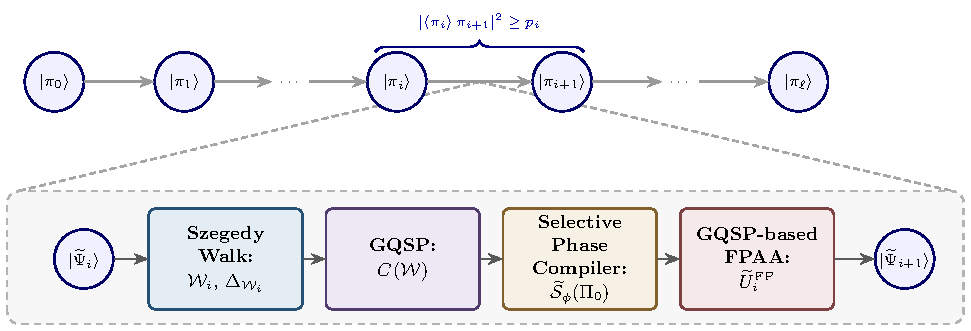
\includegraphics[width=0.95\textwidth]{qsample-validation/paper/fig0_overview.pdf}
\caption{Architecture of the constant-ancilla \textsc{QSample}
preparation algorithm. \textbf{Top row:} the cooling schedule advances
through \(\ell\) stages of stationary states
\(\ket{\pi_0}\to\cdots\to\ket{\pi_\ell}\).
\textbf{Bottom row:} each transition
\(\ket{\widetilde{\pi}_i}\to\ket{\widetilde{\pi}_{i+1}}\) uses the
qubitized Szegedy walk, to build a GQSP-based selective-phase compiler,
to then use FPAA subroutine to transport the state.}
\label{fig:qsample_overview}
\end{figure*}

\begin{figure*}[!t]
\centering
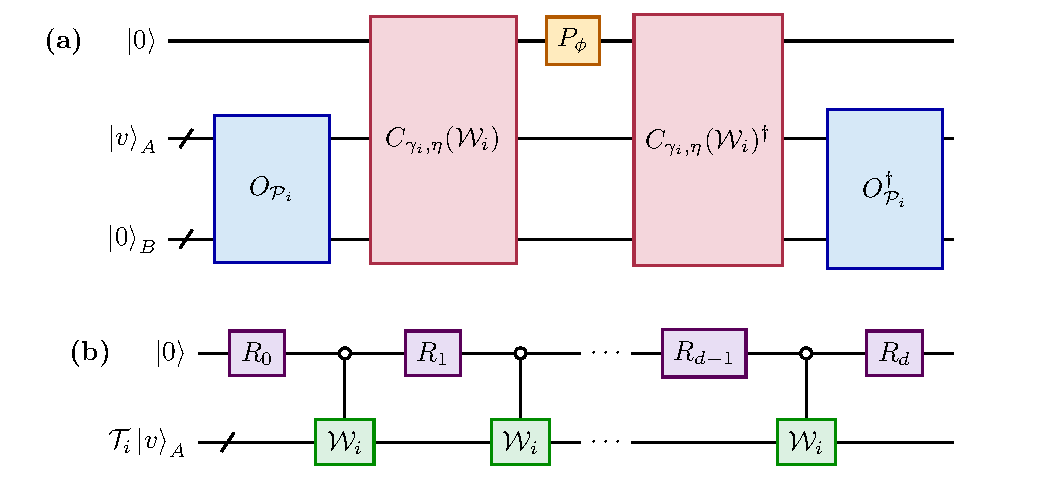
\includegraphics[width=0.94\textwidth]{qsample-validation/paper/fig1_compiler.pdf}
\caption{Complete common-interface selective-phase compiler.
(a)~The transition oracle lifts \(J\ket{v}\) into walk space, the
GQSP block computes the zero-eigenphase filter, \(P_\phi\) phases its
accepted branch, and both are uncomputed.  (b)~The one-signal-qubit
implementation of \(C_{\gamma_i,\eta}(\mathcal W_i)\) acts on the
lifted state
\(\mathcal T_i\ket{v}_A
=O_{\mathcal P_i}(\ket{v}_A\ket0_B)\) arising in (a) and uses \(d\)
zero-controlled walk calls.  Open control circles denote control on
the signal state \(\ket{0}\).  On the clean column,
\(\|\widetilde{\mathcal S}_{i,\phi}^{(\eta)}J
-J\mathcal S_\phi(\Pi_{\pi_i})\|
\leq |e^{i\phi}-1|\eta\).}
\label{fig:gadget_circuit}
\end{figure*}

\begin{definition}[Phase gap]
Let \(\mathcal{W}\) be the qubitized Szegedy walk associated with \(\mathcal{P}\). Its phase gap is
\begin{equation}
\Delta_{\mathcal{W}}
:=
\min\{|\theta|:\theta\neq 0,\ e^{i\theta}\in\mathrm{spec}(\mathcal{W}),
\ \theta\in(-\pi,\pi]\}.
\end{equation}
\end{definition}
Szegedy spectral mapping gives
\begin{align}
\Delta_{\mathcal{W}}
&= \arccos(\lambda_2(P)) \nonumber\\
&\in \Omega\left(\sqrt{\delta(\mathcal{P})}\right).
\end{align}
Let $\Pi_0$ denote the orthogonal projector onto the \(1\)-eigenspace of \(\mathcal{W}\), i.e.
$\operatorname{Im}(\Pi_0)=\ker(\mathcal{W}-\mathbb{I}).$
The full \(1\)-eigenspace can contain vectors outside the active
Szegedy subspace, so \(\Pi_0\) need not be rank one.  What the
algorithm needs is the following restricted identity.

\begin{lemma}[Stationary-space intertwining]
\label{lem:stationary-intertwining}
For a reversible ergodic chain \(\mathcal P\), with
\(\Pi_\pi:=\ket{\pi}\!\bra{\pi}\),
\begin{equation}
\Pi_0\mathcal T=\mathcal T\Pi_\pi .
\label{eq:projector-intertwining}
\end{equation}
\end{lemma}
\begin{proof}
Let \(\mathcal K:=\operatorname{Im}(\mathcal T)+
S\operatorname{Im}(\mathcal T)\).  Directly from
\(\mathcal W=(2\mathcal T\mathcal T^\dagger-\mathbb I)S\), one has
\(\mathcal W(\mathcal K)\subseteq\mathcal K\).  Since \(\mathcal W\)
is unitary on a finite-dimensional space,
\(\mathcal W(\mathcal K)=\mathcal K\); consequently \(\mathcal K\) is
reducing and \(\mathcal W(\mathcal K^\perp)=\mathcal K^\perp\).
The discriminant
\(\mathcal T^\dagger S\mathcal T\) is similar to \(P\), and
ergodicity makes its \(1\)-eigenvector \(\ket{\pi}\) unique.
Szegedy spectral mapping therefore makes
\(\ket{\psi}=\mathcal T\ket{\pi}\) the only \(1\)-eigenvector of
\(\mathcal W\) in \(\mathcal K\).  Any additional \(1\)-eigenvectors
lie in \(\mathcal K^\perp\), hence are orthogonal to
\(\operatorname{Im}(\mathcal T)\).  Projecting an arbitrary
\(\mathcal T\ket{v}\) onto the full \(1\)-eigenspace gives
\(\ket{\psi}\braket{\psi}{\mathcal T v}
=\mathcal T\ket{\pi}\braket{\pi}{v}\), proving
\eqref{eq:projector-intertwining}.
\end{proof}

Consequently, the relevant spectral decomposition is
\[
\mathcal{W}=\Pi_0+\sum_{j\geq 1}e^{i\theta_j}\Pi_j,
\qquad |\theta_j|\geq \Delta_{\mathcal{W}},
\]
and Lemma~\ref{lem:stationary-intertwining} implies
\(\mathcal S_\phi(\Pi_0)\mathcal T
=\mathcal T\mathcal S_\phi(\Pi_\pi)\).
For density operators \(\rho,\sigma\) on the same Hilbert space,
define
\begin{equation}
D_{\mathrm{tr}}(\rho,\sigma):=\frac12\|\rho-\sigma\|_1,
\end{equation}
where \(\|\cdot\|_1\) is the trace norm.  For normalized pure states,
this specializes to
\begin{equation}
D_{\mathrm{tr}}(\ket{\alpha}\!\bra{\alpha},
\ket{\beta}\!\bra{\beta})
=
\sqrt{1-|\braket{\alpha}{\beta}|^2},
\end{equation}
and \(D_{\mathrm{tr}}(\ket{\alpha},\ket{\beta})\) denotes this trace
distance between the corresponding rank-one density operators.
The total variation distance (TVD) of probability distributions
\(\alpha,\beta\) on \(\Omega\) is
\begin{equation}
d_{\mathrm{TV}}(\alpha,\beta)
:=
\frac{1}{2}\sum_{x\in\Omega}\left|\alpha(x)-\beta(x)\right|.
\end{equation}
It can be shown that $d_{\mathrm{TV}}(\alpha,\beta)
\le
D_{\mathrm{tr}}(\ket{\alpha},\ket{\beta}).$ Throughout we also denote \(\|\cdot\|\) as the operator norm.

\emph{Promised inputs and space convention.}
For every schedule stage we assume certified lower bounds on the
adjacent squared overlap and walk phase gap.  The cost of obtaining
these promises is not included; proving a useful chain-gap bound can
dominate an application, and a conservative bound directly increases
the filter degree.  ``One ancilla'' below means one clean GQSP signal
qubit beyond the two \(\Omega\)-registers.  Any workspace internal to
controlled-\(O_{\mathcal P}\), arithmetic, or classical phase
synthesis is excluded and must be added to the total implementation
width.










% ============================================================
% SECTION 3: SELECTIVE PHASE GADGET
% ============================================================

\section{Selective Phase Compiler}
\label{sec:selective-phase}

FPAA needs adjustable phases about both its source and target
states, rather than only a \(\pi\)-reflection.  For an orthogonal
projector \(\Pi\), define

\begin{definition}[Selective phase]
\label{def:selective_phase_operator}
For \(\phi\in\mathbb R\), the selective phase about
\(\operatorname{Im}(\Pi)\) is
\begin{equation}
\mathcal{S}_\phi(\Pi) := \mathbb{I} + (e^{i\phi}-1)\Pi.
\end{equation}
\end{definition}
It applies \(e^{i\phi}\) on the selected subspace and the identity on
its complement; \(\phi=\pi\) gives a reflection.

The construction has three transparent steps.  First, a one-qubit
GQSP circuit computes a block \(\Upsilon(\mathcal W)\) that is the
identity on eigenphase zero and is suppressed on phases separated by
the certified lower bound \(0<\gamma\leq\Delta_{\mathcal W}\).
Second, a phase \(P_\phi\) is applied only to the
``accepted'' signal-qubit branch and the filter is uncomputed.
Finally, Lemma~\ref{lem:stationary-intertwining} transports the
operation from the lifted walk space to \(\ket{\pi}\).  Concretely,
\begin{equation}
\label{eq:selective-phase-construction}
\widetilde{\mathcal{S}}^{\mathrm{walk}}_\phi(\Pi_0):=
C_{\gamma,\varepsilon}(\mathcal{W})^\dagger(P_\phi\otimes \mathbb{I})C_{\gamma,\varepsilon}(\mathcal{W}).
\end{equation}
Here \(P_\phi=e^{i\phi}\ket0\!\bra0+\ket1\!\bra1\).

\begin{corollary}[One-qubit GQSP filter]
\label{cor:w-spectral-filter}
For any certified \(0<\gamma\leq\Delta_{\mathcal W}\) and
\(\varepsilon^{\mathcal W}\in(0,1)\), there are
degree-\(d\) polynomials \(\Upsilon,\Phi\) and a one-signal-qubit
unitary \(C_{\gamma,\varepsilon}(\mathcal W)\) such that
\begin{align}
C_{\gamma,\varepsilon}(\mathcal W)(\ket0\otimes\mathbb I)
&=\ket0\otimes\Upsilon(\mathcal W)
 +\ket1\otimes\Phi(\mathcal W), \label{eq:gqsp-block-column}\\
\|\Upsilon(\mathcal W)-\Pi_0\|
&\leq\varepsilon^{\mathcal W}, \nonumber\\
\Upsilon(\mathcal W)^\dagger\Upsilon(\mathcal W)
&+\Phi(\mathcal W)^\dagger\Phi(\mathcal W)=\mathbb I ,
\label{eq:gqsp-filter-properties}
\end{align}
One explicit choice is
\begin{equation}
\label{eq:explicit-filter}
\begin{split}
t_\gamma&:=\left\lceil
\frac{\mathrm e}{\sin(\gamma/2)}\right\rceil,\qquad
n_\varepsilon:=\left\lceil
\ln\frac{1}{\varepsilon^{\mathcal W}}\right\rceil,\\
\Upsilon_{\gamma,\varepsilon}(z)
&:=
\left(\frac{1}{t_\gamma}
\sum_{k=0}^{t_\gamma-1}z^k\right)^{n_\varepsilon}.
\end{split}
\end{equation}
Its degree and the exact number of controlled-\(\mathcal W\) calls
in \(C_{\gamma,\varepsilon}\) are
\begin{equation}
\label{eq:explicit-filter-degree}
d=(t_\gamma-1)n_\varepsilon
=\mathcal O\!\left(
\frac{1}{\gamma}\log\frac{2}{\varepsilon^{\mathcal W}}\right).
\end{equation}
\end{corollary}

\begin{proof}
The averaged-power family follows the geometric-series filter of
Ref.~\cite{claudon2025simplealgorithmreflecteigenspaces}; the constant
in \(t_\gamma\) is chosen directly from the bound below.  The filter has
\(\Upsilon_{\gamma,\varepsilon}(1)=1\), and the triangle inequality
gives \(|\Upsilon_{\gamma,\varepsilon}(z)|\leq1\) for
\(|z|=1\).  For \(\gamma\leq|\theta|\leq\pi\),
\begin{align}
\left|
\frac{1}{t_\gamma}\sum_{k=0}^{t_\gamma-1}e^{ik\theta}
\right|
&=
\frac{|\sin(t_\gamma\theta/2)|}
{t_\gamma|\sin(\theta/2)|}\nonumber\\
&\leq
\frac{1}{t_\gamma\sin(\gamma/2)}
\leq \mathrm e^{-1}.
\label{eq:geometric-filter-bound}
\end{align}
Therefore
\(|\Upsilon_{\gamma,\varepsilon}(e^{i\theta})|
\leq\mathrm e^{-n_\varepsilon}
\leq\varepsilon^{\mathcal W}\).
Functional calculus gives
\[
\Upsilon(\mathcal W)-\Pi_0
=\sum_{j\geq1}\Upsilon(e^{i\theta_j})\Pi_j ,
\]
whose norm is at most \(\varepsilon^{\mathcal W}\).
Fej\'er--Riesz factorization of the nonnegative trigonometric
polynomial \(1-|\Upsilon|^2\) supplies a degree-at-most-\(d\)
complement \(\Phi\); the GQSP theorem then realizes
\eqref{eq:gqsp-block-column}--\eqref{eq:gqsp-filter-properties} with
exactly \(d\) controlled-\(\mathcal W\) calls and one signal qubit
\cite{MotlaghWiebe2024GQSP}.
\end{proof}

We use the zero-controlled signal convention: each controlled
\(\mathcal W\) acts when the signal is \(\ket0\), interleaved with
single-qubit rotations \(R_0,\ldots,R_d\in\mathrm{SU}(2)\).
The GQSP synthesis theorem supplies these rotations for
\(\Upsilon\); no additional phase-estimation register is introduced.

\begin{proposition}[Compiled selective phase]
\label{prop:stationary_selective_phase}
The circuit \eqref{eq:selective-phase-construction} satisfies
\begin{equation}
\label{eq:fpaa-ready-selective-phase-bound}
\begin{aligned}
&\left\|\widetilde{\mathcal{S}}^{\mathrm{walk}}_\phi(\Pi_0)
(\ket{0}\otimes \mathbb{I})\mathcal{T}
-(\ket{0}\otimes \mathbb{I})\mathcal{T}
\mathcal{S}_\phi(\Pi_\pi)\right\|\\
&\hspace{2em}\leq
2|\sin(\phi/2)|\varepsilon^{\mathcal{W}}
\leq 2\varepsilon^{\mathcal W}.
\end{aligned}
\end{equation}
It uses one signal qubit, exactly \(2d\)
controlled-\(\mathcal{W}\) or controlled-\(\mathcal W^\dagger\)
queries, and \(4d\) transition-oracle queries.  Here \(d\) is
\eqref{eq:explicit-filter-degree}; each walk query contains one
forward and one inverse transition-oracle call.
\end{proposition}
\begin{proof}
Suppress tensor-product identities and set
\(\mathcal Q:=\Upsilon(\mathcal W)^\dagger\Upsilon(\mathcal W)\).
Equation~\eqref{eq:gqsp-block-column} makes the signal-\(\ket0\)
block after compute--phase--uncompute
\begin{equation}
\begin{aligned}
\mathcal{A}
&= \bra{0}\widetilde{\mathcal{S}}^{\mathrm{walk}}_\phi(\Pi_0)\ket{0} \\
&= e^{i\phi}\Upsilon(\mathcal{W})^\dagger\Upsilon(\mathcal{W})
+ \Phi(\mathcal{W})^\dagger\Phi(\mathcal{W}) \\
&= \mathbb{I} + (e^{i\phi}-1)\mathcal{Q}.
\end{aligned}
\end{equation}
Thus the wrapper replaces the ideal projector by the positive
operator
\[
\mathcal{Q}
=
\Pi_0+\sum_{j\geq1}|\Upsilon(e^{i\theta_j})|^2\Pi_j,
\]
so \(0\leq\mathcal Q-\Pi_0\leq
(\varepsilon^{\mathcal W})^2(\mathbb I-\Pi_0)\).
Let
\(\mathcal B:=\bra1\widetilde{\mathcal S}^{\mathrm{walk}}_\phi(\Pi_0)\ket0\).
Unitarity of the first block column gives
\[
\mathcal B^\dagger\mathcal B
=\mathbb I-\mathcal A^\dagger\mathcal A
=|e^{i\phi}-1|^2(\mathcal Q-\mathcal Q^2).
\]
For
\[
\mathcal{E}_\phi
:=
\widetilde{\mathcal{S}}^{\mathrm{walk}}_\phi(\Pi_0)(\ket{0}\otimes \mathbb{I})
-
(\ket{0}\otimes \mathbb{I})\mathcal{S}_\phi(\Pi_0).
\]
the signal branches are orthogonal and
\[
\mathcal E_\phi^\dagger\mathcal E_\phi
=|e^{i\phi}-1|^2(\mathcal Q-\Pi_0).
\]
Hence
\(\|\mathcal E_\phi\|\leq
|e^{i\phi}-1|\varepsilon^{\mathcal W}
=2|\sin(\phi/2)|\varepsilon^{\mathcal W}\).
Right multiplication by the isometry \(\mathcal T\), followed by
Lemma~\ref{lem:stationary-intertwining}, proves
\eqref{eq:fpaa-ready-selective-phase-bound}.
\end{proof}

Using the clean embedding \(J\) defined in
Section~\ref{sec:preliminaries}, place the ideal and implemented
operations on the common joint space.  For chain \(j\) and accuracy
\(\eta\), let \(\Pi_{0,j}\) be the full
\(1\)-eigenspace projector of \(\mathcal W_j\), and define
\begin{equation}
\widetilde{\mathcal S}_{j,\phi}^{(\eta)}
:=
(\mathbb I_a\otimes O_{\mathcal P_j}^{\dagger})
\widetilde{\mathcal S}^{\mathrm{walk}}_{\phi}(\Pi_{0,j})
(\mathbb I_a\otimes O_{\mathcal P_j}).
\label{eq:lifted-back-compiler}
\end{equation}
The middle circuit uses \(C_{\gamma_j,\eta}(\mathcal W_j)\).
Proposition~\ref{prop:stationary_selective_phase} is equivalently the
restricted map bound
\begin{equation}
\left\|
\widetilde{\mathcal S}_{j,\phi}^{(\eta)}J
-J\mathcal S_\phi(\Pi_{\pi_j})
\right\|
\leq
2|\sin(\phi/2)|\eta.
\label{eq:clean-compiler-bound}
\end{equation}
For the corresponding degree-\(d\) filter,
\(\widetilde{\mathcal S}_{j,\phi}^{(\eta)}\) uses \(2d\) controlled
walk calls and \(4d+2\) transition-oracle calls; the final two
queries are the lift and unlift in
\eqref{eq:lifted-back-compiler}.

% ============================================================
% SECTION 4: FPAA TRANSPORT WITH APPROXIMATE PHASES
% ============================================================

\section{Fixed-Point Amplitude Amplification}
\label{sec:fpaa-transport}

FPAA transports \(\ket{\pi_i}\) to \(\ket{\pi_{i+1}}\) using only a
lower bound \(p_i\leq q_i\), avoiding over-rotation while retaining
the quadratic \(1/\sqrt{p_i}\) dependence \cite{Yoder_2014}.  In
contrast, the \(\pi/3\) fixed-point procedure analyzed in
Ref.~\cite{wocjan_speed-up_2008} scales as \(1/p_i\).

\begin{figure*}[!t]
\centering
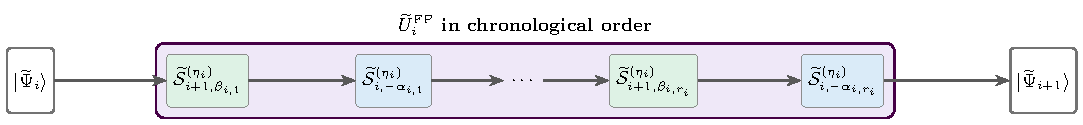
\includegraphics[width=0.98\textwidth]{qsample-validation/paper/fig2_architecture.pdf}
\caption{One FPAA transport stage in the fixed common embedding.  In
chronological order, the Yoder--Low--Chuang FPAA unitary alternates a compiled
target-chain phase
\(\widetilde{\mathcal S}_{i+1,\beta_{i,j}}^{(\eta_i)}\) with a compiled
source-chain phase
\(\widetilde{\mathcal S}_{i,-\alpha_{i,j}}^{(\eta_i)}\).
Every wrapper begins and ends in the same \(J\)-encoded space, so the
phase-dependent clean-column bounds compose without a hidden change of
register convention.}
\label{fig:qsa_architecture}
\end{figure*}

\begin{theorem}[FPAA \cite{Yoder_2014}, restated]
\label{thm:fpaa-ideal}
For \(q_i\geq p_i>0\) and
\(\varepsilon_i^{\mathrm{FP}}\in(0,1)\), choose an odd \(L_i\geq3\)
such that, with
\(\xi_i^{-1}:=T_{1/L_i}(1/\varepsilon_i^{\mathrm{FP}})\),
\begin{equation}
1-\xi_i^2\leq p_i .
\label{eq:yoder-width}
\end{equation}
Here \(T_\nu(x)=\cosh(\nu\,\operatorname{arcosh}x)\) for \(x\geq1\).
The smallest such odd sequence parameter \(L_i\) obeys
\begin{equation}
L_i = \mathcal{O}\!\left(\frac{1}{\sqrt{p_i}}\log\frac{2}{\varepsilon_i^{\mathrm{FP}}}\right)
\end{equation}
and its phases are explicit.  Writing
\(r_i=(L_i-1)/2\), for \(1\leq j\leq r_i\) take
\begin{equation}
\alpha_{i,j}=-\beta_{i,r_i-j+1}
=2\cot^{-1}\!\left[
\tan\frac{2\pi j}{L_i}\sqrt{1-\xi_i^2}\right].
\label{eq:yoder-phases}
\end{equation}
Here \(\cot^{-1}\colon\mathbb R\to(0,\pi)\) denotes the principal
arccotangent, and phases are understood modulo \(2\pi\).
Set
\(V_{i,2j-1}:=\mathcal S_{\beta_{i,j}}(\Pi_{\pi_{i+1}})\)
and
\(V_{i,2j}:=\mathcal S_{-\alpha_{i,j}}(\Pi_{\pi_i})\).
Then, with \(m_i:=L_i-1\),
\begin{equation}
U_i^{\mathrm{FP}}:=V_{i,m_i}\cdots V_{i,1}
\end{equation}
satisfies
\[
D_{\mathrm{tr}}\bigl(U_i^{\mathrm{FP}}\ket{\pi_i},
\ket{\pi_{i+1}}\bigr)\leq\varepsilon_i^{\mathrm{FP}}.
\]
Products act right-to-left: in every pair the target phase
\(V_{i,2j-1}\) acts first and the source phase \(V_{i,2j}\) second,
matching the generalized Grover iterate of Ref.~\cite{Yoder_2014}
up to its irrelevant global minus sign.
\end{theorem}

\begin{corollary}[Phase-weighted compiled FPAA]
\label{cor:gqsp_fpaa}
Choose \(L_i\) and its phases as in
Theorem~\ref{thm:fpaa-ideal}.  Replace every \(V_{i,k}\) by its
lifted-back compiler \(\widetilde V_{i,k}\).  Let the source filter in
pair \(j\) have accuracy \(\eta_{i,j}^{\rm s}\), and the target
filter have accuracy \(\eta_{i,j}^{\rm t}\).  Set
\(\widetilde U_i^{\mathrm{FP}}
:=\widetilde V_{i,m_i}\cdots\widetilde V_{i,1}\).  Then
\begin{align}
D_{\mathrm{tr}}\left(
\widetilde U_i^{\mathrm{FP}}J\ket{\pi_i},
J\ket{\pi_{i+1}}\right)
&\leq\varepsilon_i^{\mathrm{FP}}
+2\sum_{j=1}^{r_i}
\left|\sin\frac{\alpha_{i,j}}2\right|\eta_{i,j}^{\rm s}
\nonumber\\
&\quad
+2\sum_{j=1}^{r_i}
\left|\sin\frac{\beta_{i,j}}2\right|\eta_{i,j}^{\rm t}.
\label{eq:phase-weighted-fpaa}
\end{align}
\end{corollary}

\begin{proof}
The clean-column estimate is not a global operator bound, so we
hybridize through ideal clean prefixes.  Let
\(\widetilde V_{>k}:=\widetilde V_{i,m_i}\cdots
\widetilde V_{i,k+1}\) and
\(V_{<k}:=V_{i,k-1}\cdots V_{i,1}\), with empty products equal to
the identity.  Then the exact identity
\[
\widetilde U_i^{\mathrm{FP}}J-JU_i^{\mathrm{FP}}
=\sum_{k=1}^{m_i}
\widetilde V_{>k}(\widetilde V_{i,k}J-JV_{i,k})V_{<k}
\]
is well typed on the common joint space.  All outer factors are
unitary, and \eqref{eq:clean-compiler-bound} applies because the
right prefix is ideal and therefore remains in the clean image of
\(J\).  Applying its phase-dependent bound separately to every
source and target phase gives the sum in
\eqref{eq:phase-weighted-fpaa}.
Trace distance between the corresponding pure joint states is no
larger than their vector distance.  The triangle inequality and
Theorem~\ref{thm:fpaa-ideal} complete the proof.
\end{proof}

For later use, define the computable phase weight
\begin{equation}
\label{eq:phase-weight}
A_i:=
\sum_{j=1}^{r_i}\left(
\left|\sin\frac{\alpha_{i,j}}2\right|
+\left|\sin\frac{\beta_{i,j}}2\right|\right)
\leq L_i-1.
\end{equation}
Indeed, with \(s_i:=\sqrt{1-\xi_i^2}\leq1\), phase-list symmetry and
the \(j=r_i\) term give
\(A_i\geq2[1+s_i^2\tan^2(\pi/L_i)]^{-1/2}
\geq2\cos(\pi/L_i)\geq1\); hence \(\eta_i\in(0,1)\).
If all filters at stage \(i\) use accuracy \(\eta_i\),
Corollary~\ref{cor:gqsp_fpaa} becomes
\(D_{\rm tr}\leq\varepsilon_i^{\rm FP}+2A_i\eta_i\).

% ============================================================
% SECTION 5: END-TO-END FRAMEWORK
% ============================================================

\section{End-to-End \textsc{QSample} Preparation Framework}
\label{sec:end-to-end}

At stage \(i\), FPAA alternates lifted-back compilers for chains
\(i\) and \(i+1\); it is not a single pass through two reflections.
The same signal qubit and transition register are reused throughout.
Algorithm~\ref{alg:qsample_gqsp} exposes the required classical
promises and the error allocation.

\begin{algorithm}[!ht]
\caption{\textsc{QSample} Preparation}
\label{alg:qsample_gqsp}
\KwIn{Controlled circuits
\(\{O_{\mathcal P_i},O_{\mathcal P_i}^\dagger\}_{i=0}^{\ell}\);
certified \(p_i>0\) with
\(|\braket{\pi_i}{\pi_{i+1}}|^2\geq p_i\) for \(i<\ell\) and
\(\Delta_{\mathcal W_j}\geq\gamma_j>0\) for \(j\leq\ell\);
\(\ket{\pi_0}\); error \(\varepsilon\in(0,1)\).}
\KwOut{Joint state \(\ket{\widetilde\Psi_\ell}\) satisfying
\(D_{\rm tr}(\ket{\widetilde\Psi_\ell},J\ket{\pi_\ell})
\le\varepsilon\).}
Initialize \(\ket{\widetilde\Psi_0}\leftarrow J\ket{\pi_0}\)\;
\For{$i \leftarrow 0$ \KwTo $\ell-1$}{
Set \(\varepsilon_i=\varepsilon/\ell\) and
\(\varepsilon_i^{\rm FP}=\varepsilon_i/2\), then choose the smallest
odd \(L_i\ge3\) satisfying \eqref{eq:yoder-width} and compute its phases\;
Compute \(A_i\) from \eqref{eq:phase-weight} and set
\(\eta_i=\varepsilon_i/(4A_i)\)\;
Synthesize the \(i\) and \(i+1\) filters using
\(\gamma_i,\gamma_{i+1}\) and accuracy \(\eta_i\)\;
\(\ket{\widetilde\Psi_{i+1}}\leftarrow
\widetilde U_i^{\rm FP}\ket{\widetilde\Psi_i}\)\;
}
\Return \(\ket{\widetilde\Psi_\ell}\)\;
\end{algorithm}

For the explicit filter \eqref{eq:explicit-filter}, define the
stage-\(i\), chain-\(j\) degree
\begin{equation}
\label{eq:stage-filter-degree}
d_{i,j}:=
\left(\left\lceil\frac{\mathrm e}{\sin(\gamma_j/2)}\right\rceil-1\right)
\left\lceil\ln\frac1{\eta_i}\right\rceil,
\qquad j\in\{i,i+1\}.
\end{equation}
Counting each forward or inverse use of \(O_{\mathcal P_j}\), controlled when
required, as one transition-oracle query, stage \(i\) uses exactly
\begin{equation}
\label{eq:exact-stage-queries}
Q_i=2(L_i-1)\bigl(d_{i,i}+d_{i,i+1}+1\bigr)
\end{equation}
queries, including every lift and unlift.

\begin{theorem}[End-to-end preparation]
\label{thm:end-to-end}
Let \(\ell\geq1\), let \(\varepsilon\in(0,1)\), and let
\(\{\mathcal P_i\}_{i=0}^{\ell}\) be reversible ergodic chains on
\(\Omega\), with stationary \textup{\textsc{QSamples}}
\(\ket{\pi_i}\).
Suppose that, for \(0\leq i<\ell\),
\begin{equation}
q_i:=|\braket{\pi_i}{\pi_{i+1}}|^2\geq p_i>0,
\end{equation}
and that \(\Delta_{\mathcal W_i}\geq\gamma_i>0\) for
\(0\leq i\leq\ell\), where \(p_i,\gamma_i\) are supplied certified
bounds.  Define
\[
\gamma_i^\star:=\min\{\gamma_i,\gamma_{i+1}\},\quad
p_{\min}:=\min_{i<\ell}p_i,\quad
\gamma_{\min}:=\min_{i\leq\ell}\gamma_i .
\]
Given exact preparation of \(\ket{\pi_0}\) and coherently
controllable circuits \(O_{\mathcal P_i},O_{\mathcal P_i}^\dagger\), Algorithm
\ref{alg:qsample_gqsp} produces a joint pure state
\(\ket{\widetilde\Psi_\ell}\) such that
\begin{equation}
D_{\rm tr}\!\left(
\ket{\widetilde\Psi_\ell},J\ket{\pi_\ell}\right)\leq\varepsilon .
\label{eq:joint-output-guarantee}
\end{equation}
Its transition-oracle query count, with control when required, is
\begin{equation}
\label{eq:query_complexity_main_sum}
\mathcal O\!\left(
\sum_{i=0}^{\ell-1}
\frac{\log(4\ell/\varepsilon)}
{\sqrt{p_i}\,\gamma_i^\star}
\log\!\left(
\mathrm e+
\frac{\ell}{\varepsilon\sqrt{p_i}}
\log\frac{4\ell}{\varepsilon}
\right)\right).
\end{equation}
In particular, this is
\[
\widetilde{\mathcal O}\!\left(
\frac{\ell}{\sqrt{p_{\min}}\,\gamma_{\min}}\right).
\]
If
\(\widetilde\rho_\ell:=
\operatorname{Tr}_{aB}
\ket{\widetilde\Psi_\ell}\!\bra{\widetilde\Psi_\ell}\),
then
\[
D_{\rm tr}(\widetilde\rho_\ell,
\ket{\pi_\ell}\!\bra{\pi_\ell})\leq\varepsilon ,
\qquad
\TV(\widetilde\pi_\ell,\pi_\ell)\leq\varepsilon ,
\]
where \(\widetilde\pi_\ell\) is the outcome distribution obtained by
measuring \(A\).  Outside oracle-internal scratch space, the peak
width is \(2\lceil\log_2|\Omega|\rceil+1\) qubits.
\end{theorem}

\begin{proof}
Set \(\varepsilon_i=\varepsilon/\ell\),
\(\varepsilon_i^{\rm FP}=\varepsilon_i/2\), and
\(\eta_i=\varepsilon_i/(4A_i)\).
Corollary~\ref{cor:gqsp_fpaa} gives
\[
D_{\rm tr}\!\left(
\widetilde U_i^{\rm FP}J\ket{\pi_i},J\ket{\pi_{i+1}}\right)
\leq\varepsilon_i .
\]
Theorem~\ref{thm:fpaa-ideal}, with
\(\varepsilon_i^{\rm FP}=\varepsilon/(2\ell)\), gives
\[
L_i=\mathcal O\!\left(
p_i^{-1/2}\log\frac{4\ell}{\varepsilon}\right).
\]
Each compiled phase uses the \(i\)- or \(i+1\)-chain filter and
therefore
\[
\mathcal O\!\left(
\frac{1}{\gamma_i^\star}
\log\frac{1}{\eta_i}\right)
\]
controlled walks.  Since \(\eta_i=\varepsilon/(4\ell A_i)\) and
\(A_i\leq L_i-1\), \(\log(1/\eta_i)=\log(4\ell A_i/\varepsilon)\) is
\[
\mathcal O\!\left(\log\!\left(
\mathrm e+\frac{\ell}{\varepsilon\sqrt{p_i}}
\log\frac{4\ell}{\varepsilon}\right)\right).
\]
Multiplying by \(L_i-1\) and
summing the stages yields \eqref{eq:query_complexity_main_sum}.
Equation~\eqref{eq:exact-stage-queries} gives the corresponding
constant-resolved count for the explicit filter.

For the actual recurrence
\(\ket{\widetilde\Psi_{i+1}}
:=\widetilde U_i^{\rm FP}\ket{\widetilde\Psi_i}\), unitary invariance
and the triangle inequality give
\[
\begin{aligned}
D_{\rm tr}(\ket{\widetilde\Psi_{i+1}},J\ket{\pi_{i+1}})
&\leq
D_{\rm tr}(\ket{\widetilde\Psi_i},J\ket{\pi_i})
+\varepsilon_i .
\end{aligned}
\]
The initial term is zero, proving
\eqref{eq:joint-output-guarantee} by induction.  Contractivity under
partial trace gives the system-register statement, and
contractivity under measurement gives the TVD statement.  The walk
uses two \(\Omega\)-registers and the compiler reuses one signal
qubit; any workspace inside the supplied oracle circuits is excluded.
\end{proof}

\FloatBarrier
\begin{table}[!t]
\caption{Fixed-schedule comparison with the coherent-QPE/\(\pi/3\)
construction of Ref.~\cite{wocjan_speed-up_2008}.}
\label{tab:comparison}
\centering
\footnotesize
\renewcommand{\arraystretch}{1.3}
\setlength{\tabcolsep}{3pt}
\begin{tabular}{@{}lcc@{}}
\toprule
& \textbf{Ref.~\cite{wocjan_speed-up_2008}} & \textbf{This work} \\
\midrule
Queries
& $\widetilde{\mathcal{O}}\!\left(\dfrac{\ell}{p_{\min}\gamma_{\min}}\right)$
& $\widetilde{\mathcal{O}}\!\left(\dfrac{\ell}{\sqrt{p_{\min}}\,\gamma_{\min}}\right)$ \\
Szegedy-walk qubits
& \(2\lceil\log_2|\Omega|\rceil\)
& \(2\lceil\log_2|\Omega|\rceil\) \\
Ancilla overhead
& $\mathcal{O}\!\left(\log\dfrac{1}{\gamma_{\min}}\log\dfrac{\ell}{\varepsilon p_{\min}}\right)$
& $1$ \\
Oracle-internal scratch
& excluded & excluded \\
\bottomrule
\end{tabular}
\end{table}

\noindent
Here one query is one forward or inverse use of \(O_{\mathcal P_i}\),
controlled when required, and both columns exclude
oracle-internal scratch space.  The comparison holds the prescribed
schedule and access model fixed: schedule refinement may exchange a
larger \(\ell\) for better adjacent overlaps.  Single-ancilla
iterative QPE and coherent low-ancilla phase-estimation alternatives
exist \cite{Dobsicek2007,Rall2021}; Table~\ref{tab:comparison} concerns
the particular coherent-QPE reflection analyzed in
Ref.~\cite{wocjan_speed-up_2008}.

\subsection{A regime with subconstant adjacent overlap}
\label{sec:subconstant-overlap}
The improvement over the Ref.~\cite{wocjan_speed-up_2008}
\(1/p_i\) bound is asymptotic outside the well-balanced schedule used
in Section~\ref{sec:application}.  Consider
\(\Omega=\{0,1\}^n\) and
\(H(x)=\sum_{k=1}^n x_k\).  Its Gibbs distribution is
\(\mu_\beta=\operatorname{Ber}(r_\beta)^{\otimes n}\), where
\(r_\beta=(1+\mathrm e^\beta)^{-1}\).  Between \(\beta=0\) and
\(\beta>0\), the squared \textsc{QSample} overlap is
\begin{equation}
\label{eq:product-gibbs-overlap}
q(\beta)=
\left[\frac{1+\operatorname{sech}(\beta/2)}{2}\right]^n .
\end{equation}
For \(n\geq2\), choose
\begin{equation}
\label{eq:product-gibbs-beta}
\beta_n=
2\operatorname{arcosh}\!\left(
\frac{1}{2n^{-1/n}-1}\right)
=4\sqrt{\frac{\ln n}{n}}\left(
1+\mathcal O\!\left(\frac{\ln n}{n}\right)\right).
\end{equation}
Then \(q(\beta_n)=1/n\) exactly; take \(p_0=q(\beta_n)\).

Let \(\mathcal P_\beta\) be the lazified random-scan heat-bath chain
with transition matrix \(P_\beta=(I+G_\beta)/2\).  In the
\(\mu_\beta\)-orthogonal product basis, a mode
supported on \(S\subseteq[n]\) has eigenvalue
\(1-|S|/(2n)\); hence
\begin{equation}
\delta(\mathcal P_\beta)=\frac1{2n},\qquad
\Delta_{\mathcal W_\beta}
=\arccos\!\left(1-\frac1{2n}\right)
=\Theta(n^{-1/2})
\label{eq:product-gibbs-gap}
\end{equation}
at both endpoints.  On this one-stage schedule, the upper bound of
Ref.~\cite{wocjan_speed-up_2008} is
\(\widetilde{\mathcal O}(n^{3/2})\), whereas
Theorem~\ref{thm:end-to-end} gives
\(\widetilde{\mathcal O}(n)\).  This product model transparently
separates the Ref.~\cite{wocjan_speed-up_2008} upper bound from the
present GQSP/FPAA upper bound.  The transition oracle
is not a target-state oracle: from \(x\), a row is supported only on
\(x\) and its \(n\) one-bit neighbors, whereas \(\mu_{\beta_n}\) has
full support.  Nevertheless, this is not a query lower bound or a
claim of sampling hardness: its target
\textsc{QSample} can independently be prepared by single-qubit
rotations.

\subsection{Full-state small-instance validation}
\label{sec:numerical-validation}
We use the open \(2\times4\) ladder with ten edges,
\[
H(x)=\sum_{(u,v)\in E}\mathbf 1[x_u\neq x_v],
\]
Configurations use row-major lexicographic bit ordering.  The
inverse-temperature schedule is \(0,0.3,0.6,0.9,1.2\).
This disagreement-count normalization is equivalent, up to an additive constant, to the
conventional \(-J\sum_{(u,v)}s_us_v\) Hamiltonian with \(J=1/2\).
Random-scan heat-bath dynamics chooses one of eight sites uniformly
and resamples it from its exact conditional Gibbs law.  Its lazified
chain is \(\mathcal P_\beta\), with transition matrix
\(P_\beta=(I+G_\beta)/2\).

All \(2^8\) configurations are enumerated.  To fix the transition
oracle away from its promised clean column, set
\(\ket{p_x}:=\sum_y\sqrt{P(x,y)}\ket y\) and use the deterministic
row-wise Householder extension
\begin{equation}
\begin{aligned}
O_{\mathcal P}&=\sum_x\ket x\!\bra x\otimes H_x,\\
H_x&=I-2\ket{u_x}\!\bra{u_x},\\
\ket{u_x}&=\frac{\ket0-\ket{p_x}}
{\|\ket0-\ket{p_x}\|}.
\end{aligned}
\end{equation}
with \(H_x=I\) when the denominator vanishes.  Across the five
chains, the maximum row-sum, stationarity, detailed-balance, and
projector-intertwining operator-norm residuals are respectively
\(4.44\times10^{-16}\), \(1.39\times10^{-17}\),
\(1.08\times10^{-19}\), and \(1.70\times10^{-14}\).

For \(\varepsilon=10^{-3}\), the phase-weighted allocation gives
\(L_i=5\), \(A_i=2.28249\),
\(\varepsilon_i^{\rm FP}=1.25\times10^{-4}\), and
\(\eta_i=2.73824\times10^{-5}\) at every stage.
For table compactness, write
\(\delta_i:=\delta(\mathcal P_{\beta_i})\) and
\(\Delta_i:=\Delta_{\mathcal W_i}\).
Table~\ref{tab:exact-benchmark} reports the resulting degrees,
stagewise errors, and every controlled-walk, outer lift/unlift, and
total transition-oracle call.
Every table and figure distance and leakage value follows the approximate
compiled phases \(\widetilde{\mathcal S}_{i,\phi}^{(\eta_i)}\);
ideal projectors are used only for sequence design and an audit control.

\begin{table*}[!t]
\caption{Fully enumerated open $2\times4$ disagreement-count Ising benchmark. Panel (a) gives the stage inputs. Panel (b) fixes $\varepsilon=10^{-3}$, $\varepsilon_i^{\rm FP}=1.25\times10^{-4}$, and $A_i=2.28249$, and reports full-state propagation under the approximate compiled phases $\widetilde{\mathcal S}$. The ideal projectors are used only for sequence design and an audit control. $N_{\rm cW}$ counts controlled walk calls, $N_{\rm wrap}$ counts outer $O_{\mathcal P_j}^{(\dagger)}$ calls, and $Q_i=2N_{\rm cW}+N_{\rm wrap}$. $\widetilde D_i^{\rm local}$ starts stage $i$ from a fresh $\mathcal J\lvert\pi_i\rangle$; $\widetilde D_i^{\rm cum}$ compares the sequential prefix through stage $i$ with $\mathcal J\lvert\pi_{i+1}\rangle$.}
\label{tab:exact-benchmark}
\centering
\footnotesize
\textbf{(a) Stage inputs.}\quad
\setlength{\tabcolsep}{4.3pt}
\begin{tabular}{@{}cccccc@{}}
\toprule
$i$ & $\beta_i\!\to\!\beta_{i+1}$ & $p_i=q_i$ & $(\delta_i,\delta_{i+1})$ & $(\Delta_i,\Delta_{i+1})$ & $L_i$\\
\midrule
0 & $0.0\!\to\!0.3$ & $0.944415$ & $(0.062500,0.039040)$ & $(0.355421,0.280346)$ & $5$\\
1 & $0.3\!\to\!0.6$ & $0.939133$ & $(0.039040,0.021008)$ & $(0.280346,0.205340)$ & $5$\\
2 & $0.6\!\to\!0.9$ & $0.933454$ & $(0.021008,0.009999)$ & $(0.205340,0.141532)$ & $5$\\
3 & $0.9\!\to\!1.2$ & $0.936311$ & $(0.009999,0.004360)$ & $(0.141532,0.093413)$ & $5$\\
\bottomrule
\end{tabular}
\\[2pt]
\textbf{(b) Compiled transport.}\quad
\setlength{\tabcolsep}{3.4pt}
\begin{tabular}{@{}ccccccccc@{}}
\toprule
$i$ & $(d_{i,i},d_{i,i+1})$ & $\eta_i$ & $\widetilde D_i^{\rm local}$ & $\widetilde D_i^{\rm cum}$ & $N_{\rm cW}$ & $N_{\rm wrap}$ & $Q_i$ & leakage\\
\midrule
0 & $(165,209)$ & $2.74\!\times\!10^{-5}$ & $1.22\!\times\!10^{-4}$ & $1.22\!\times\!10^{-4}$ & $1496$ & $8$ & $3000$ & $<2.3\!\times\!10^{-15}$\\
1 & $(209,286)$ & $2.74\!\times\!10^{-5}$ & $1.04\!\times\!10^{-4}$ & $8.18\!\times\!10^{-5}$ & $1980$ & $8$ & $3968$ & $<2.3\!\times\!10^{-15}$\\
2 & $(286,418)$ & $2.74\!\times\!10^{-5}$ & $6.37\!\times\!10^{-5}$ & $6.41\!\times\!10^{-5}$ & $2816$ & $8$ & $5640$ & $<2.3\!\times\!10^{-15}$\\
3 & $(418,638)$ & $2.74\!\times\!10^{-5}$ & $8.66\!\times\!10^{-5}$ & $1.08\!\times\!10^{-4}$ & $4224$ & $8$ & $8456$ & $<2.3\!\times\!10^{-15}$\\
\bottomrule
\end{tabular}
\end{table*}


\begin{figure*}[!t]
\centering
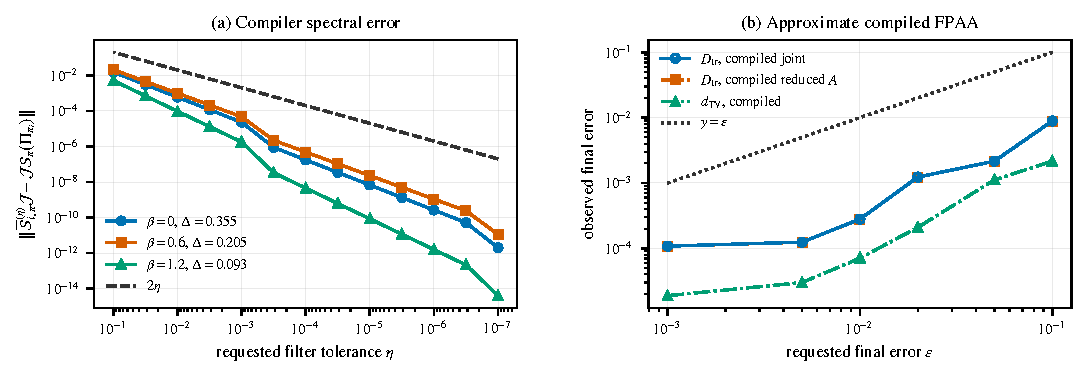
\includegraphics[width=0.98\textwidth]{qsample-validation/outputs/figures/fig3_validation.pdf}
\caption{Deterministic double-precision validation of the
fixed-completion polynomial-block reference.  (a) The restricted compiler error for
\(\phi=\pi\), evaluated on every nonstationary eigenphase of three
benchmark walks, remains below the analytic \(2\eta\) envelope.
(b) Sequential full-state propagation through all four approximate
compiled-phase FPAA stages reports joint trace distance, the full
reduced-\(A\) trace distance, and output TVD; all remain below the
requested final error.}
\label{fig:numerical-validation}
\end{figure*}

With
\(\ket{\overline{\Psi}_{i+1}}:=\ket{\widetilde\Psi_{i+1}}/
\|\widetilde\Psi_{i+1}\|_2\), the leakage probability is
\(\lambda_i^{\rm leak}:=\sum_{a,x,y:\,(a,y)\ne(0,0)}
|\langle a,x,y|\overline{\Psi}_{i+1}\rangle|^2\),
which is evaluated as a sum of nonnegative terms rather than by subtraction.
Binary64 values at or below \(10\epsilon_{\rm mach}\), with
\(\epsilon_{\rm mach}=2^{-52}\), are shown as
\(<2.3\times10^{-15}\).

We then propagate the complete state in
\(\mathbb C^2\otimes\mathbb C^{256}\otimes\mathbb C^{256}\) through
every lift, filter, conditional phase, unfilter, unlift, and FPAA
stage.  Walk functions are applied from the discriminant spectrum,
without forming the dense \(65536\times65536\) walk.  To make
off-clean signal dynamics deterministic, the reference fixes, at
each eigenvalue \(z\), the unitary scalar completion
\[
C(z)=
\begin{pmatrix}
\Upsilon(z)&-\sqrt{1-|\Upsilon(z)|^2}\\
\sqrt{1-|\Upsilon(z)|^2}&\overline{\Upsilon(z)}
\end{pmatrix}.
\]
This is a full-state spectral reference for the intended polynomial
block, not an angle-level GQSP circuit simulation; the theorem's
error envelope is independent of this completion.

At \(\varepsilon=10^{-3}\), the final joint and reduced trace
distances are both \(1.082\times10^{-4}\), the measured-system TVD is
\(1.889\times10^{-5}\), the clean-subspace leakage probability is
below the \(2.3\times10^{-15}\) reporting threshold, and the
propagated-state norm residual is \(2.29\times10^{-14}\).  The
ideal-projector control gives \(1.0816783746\times10^{-4}\), while the
compiled-to-ideal full-state distance is \(1.0847510\times10^{-8}\).
The
\texttt{qsample-validation} code, data, and scripts were used to
generate the reported data.  The routines use double-precision
diagonalization rather than interval arithmetic; finite-precision
GQSP rotation-synthesis error is excluded.  The actual-phase hybrid
bounds total \(7.6122\times10^{-7}\) versus a \(5\times10^{-4}\)
allocation; this is one exact-promise instance, not an empirical
scaling test.

% ============================================================
% SECTION 6: APPLICATION
% ============================================================

\section{Application: Classical Gibbs \textsc{QSample}}
\label{sec:application}

For a classical Hamiltonian \(H:\Omega_\mu\to\mathbb R\), let
\begin{equation}
\mu_\beta(x):=\frac{e^{-\beta H(x)}}{\mathcal Z(\beta)},
\qquad
\mathcal Z(\beta):=\sum_xe^{-\beta H(x)},
\label{eq:gibbs-distribution-general}
\end{equation}
and
\(\ket{\mu_\beta}:=\sum_x\sqrt{\mu_\beta(x)}\ket{x}\).

\begin{corollary}[Classical Gibbs \textsc{QSample}]
\label{cor:gibbs-qsampling}
Let \(n\geq2\), let \(H:\Omega_\mu\to\{0,\ldots,n\}\), fix a target inverse
temperature \(\beta_\star\), and suppose we are supplied a schedule
\[
0=\beta_0<\cdots<\beta_\ell=\beta_\star,\qquad
\ell=\mathcal O\!\left(
\sqrt{\ln|\Omega_\mu|\,\ln n}\right),
\]
obeying the well-balanced guarantee of
Ref.~\cite{Arunachalam_2022}.  For each \(i\), assume a reversible
chain \(\mathcal P_{\beta_i}\), with transition matrix \(P_{\beta_i}\)
and stationary distribution \(\mu_{\beta_i}\),
a coherently controllable transition circuit, and a certified walk
phase-gap lower bound \(\gamma_i\).  Assume also exact preparation of
the uniform initial state
\(\ket{\mu_0}=|\Omega_\mu|^{-1/2}\sum_{x\in\Omega_\mu}\ket{x}\).
Then Algorithm~\ref{alg:qsample_gqsp} prepares a joint state whose
reduced system state is
within trace distance \(\varepsilon\) of
\(\ket{\mu_{\beta_\star}}\), using
\begin{equation}
\widetilde{\mathcal O}\!\left(
\frac{\sqrt{\ln|\Omega_\mu|\,\ln n}}{\gamma_{\min}}\right)
\label{eq:gibbs-complexity}
\end{equation}
transition-oracle queries, controlled when required, and one signal
qubit beyond the two \(\Omega_\mu\)-registers, excluding oracle scratch.
\end{corollary}
\begin{proof}
The adjacent squared overlap is
\[
|\braket{\mu_{\beta_i}}{\mu_{\beta_{i+1}}}|^2
=
\frac{\mathcal Z((\beta_i+\beta_{i+1})/2)^2}
{\mathcal Z(\beta_i)\mathcal Z(\beta_{i+1})}
\geq\frac1{15}
\]
for the schedule of Ref.~\cite{Arunachalam_2022}.  Thus
\(p_i=1/15\) may be taken at every stage, so \(p_{\min}=1/15\), and
\eqref{eq:gibbs-complexity} follows directly
from Theorem~\ref{thm:end-to-end}.  Constructing the schedule and
certifying the chain gaps are separate costs and are not included.
\end{proof}

If certified classical spectral-gap bounds satisfy
\(0<\underline\delta_i\leq\delta(\mathcal P_{\beta_i})\) for
\(0\leq i\leq\ell\), then
\(\lambda_2(P_{\beta_i})\leq1-\underline\delta_i\), so one may choose
\(\gamma_i:=\arccos(1-\underline\delta_i)
\leq\Delta_{\mathcal W_i}\).
Since \(1-\cos\theta\leq\theta^2/2\),
\(1/\gamma_i\leq1/\sqrt{2\underline\delta_i}
=\mathcal O(1/\sqrt{\underline\delta_i})\).  Writing
\(\underline\delta_{\min}:=\min_{0\leq i\leq\ell}
\underline\delta_i\), \eqref{eq:gibbs-complexity} therefore becomes
\(\widetilde{\mathcal O}(
\sqrt{\ln|\Omega_\mu|\ln n}/\sqrt{\underline\delta_{\min}})\).
Because \(p_{\min}\) is constant here, replacing
\(1/p_{\min}\) by \(1/\sqrt{p_{\min}}\) changes only a constant.
The Gibbs corollary's asymptotic advantage over the
Ref.~\cite{wocjan_speed-up_2008} instantiation is therefore its
smaller additional working register.

Preparing a mixed Gibbs state of a noncommuting quantum Hamiltonian
is distinct.  Detailed-balance and KMS-Lindbladian samplers address it
under Hamiltonian and jump-operator access
\cite{ChenEtAl2025Thermal,ChenKastoryanoGilyen,DingLiLin2025}; their
costs depend on Lindbladian simulation and mixing, ours on
classical-chain transition oracles, adjacent \textsc{QSample}
overlaps, and Szegedy phase gaps, so they are not direct resource
competitors.

% ============================================================
% SECTION 7: DISCUSSION
% ============================================================

\section{Discussion and Limitations}
\label{sec:discussion}

The contribution is a one-signal-qubit GQSP realization of adjustable
stationary-state phases with higher-rank intertwining,
phase-sensitive clean-column analysis, and exact schedule accounting.
Relative to Ref.~\cite{wocjan_speed-up_2008}, it reduces signal
workspace; the improved \(p_{\min}\)-dependence is asymptotic only
when \(p_{\min}=o(1)\).

The guarantees assume controllable transition circuits, certified
overlap and phase-gap bounds, and an exact initial \textsc{QSample};
gap certification and oracle arithmetic may dominate.  The numerical
reference fixes a pointwise unitary completion but synthesizes neither
the complementary GQSP polynomial nor finite-precision angles, whose
costs fault-tolerant estimates must add.  Future work includes removing
the promises, jointly optimizing schedule and transport, and extending
the compiler to nonreversible chains \cite{Claudon_nonreversible2025}.

\IEEEtriggeratref{4}
\begin{thebibliography}{00}
\bibitem{Brassard_2002} G. Brassard, P. H{\o}yer, M. Mosca, and A. Tapp, ``Quantum amplitude amplification and estimation,'' in \emph{Quantum Computation and Information}, S. J. Lomonaco, Jr. and H. E. Brandt, Eds., \emph{Contemporary Mathematics}, vol. 305. Providence, RI, USA: American Mathematical Society, 2002, pp. 53--74. doi: \href{https://doi.org/10.1090/conm/305/05215}{10.1090/conm/305/05215}.
\bibitem{montanaro_quantum_2015} A. Montanaro, ``Quantum speedup of Monte Carlo methods,'' \emph{Proc. R. Soc. A: Math. Phys. Eng. Sci.}, vol. 471, no. 2181, Art. no. 20150301, Sep. 2015. doi: \href{https://doi.org/10.1098/rspa.2015.0301}{10.1098/rspa.2015.0301}.
\bibitem{Cornelissen_2022} A. Cornelissen, Y. Hamoudi, and S. Jerbi, ``Near-optimal quantum algorithms for multivariate mean estimation,'' in \emph{Proc. 54th Annu. ACM SIGACT Symp. Theory of Computing (STOC '22)}, ACM, Jun. 2022, pp. 33--43. doi: \href{https://doi.org/10.1145/3519935.3520045}{10.1145/3519935.3520045}.
\bibitem{wocjan_speed-up_2008} P. Wocjan and A. Abeyesinghe, ``Speedup via quantum sampling,'' \emph{Physical Review A}, vol. 78, no. 4, Art. no. 042336, Oct. 2008. doi: \href{https://doi.org/10.1103/PhysRevA.78.042336}{10.1103/PhysRevA.78.042336}.
\bibitem{Somma_2007} R. D. Somma, S. Boixo, H. Barnum, and E. Knill, ``Quantum simulations of classical annealing processes,'' \emph{Physical Review Letters}, vol. 101, no. 13, p. 130504, 2008. doi: \href{https://doi.org/10.1103/PhysRevLett.101.130504}{10.1103/PhysRevLett.101.130504}. arXiv:\href{https://arxiv.org/abs/0804.1571}{0804.1571}.
\bibitem{Szegedy2004} M. Szegedy, ``Quantum speed-up of Markov chain based algorithms,'' in \emph{Proc. 45th Annu. IEEE Symp. Foundations of Computer Science (FOCS)}, 2004, pp. 32--41. doi: \href{https://doi.org/10.1109/FOCS.2004.53}{10.1109/FOCS.2004.53}.
\bibitem{Somma_2008} R. D. Somma, S. Boixo, H. Barnum, and E. Knill, ``Quantum simulations of classical annealing processes,'' \emph{Physical Review Letters}, vol. 101, no. 13, Art. no. 130504, Sep. 2008. doi: \href{https://doi.org/10.1103/PhysRevLett.101.130504}{10.1103/PhysRevLett.101.130504}. arXiv:\href{https://arxiv.org/abs/0804.1571}{0804.1571}.
\bibitem{Magniez_2011} F. Magniez, A. Nayak, J. Roland, and M. Santha, ``Search via quantum walk,'' \emph{SIAM Journal on Computing}, vol. 40, no. 1, pp. 142--164, Jan. 2011. doi: \href{https://doi.org/10.1137/090745854}{10.1137/090745854}.
\bibitem{SVV} D. \v{S}tefankovi\v{c}, S. Vempala, and E. Vigoda, ``Adaptive simulated annealing: A near-optimal connection between sampling and counting,'' \emph{J. ACM}, vol. 56, no. 3, art. 18, May 2009. doi: \href{https://doi.org/10.1145/1516512.1516520}{10.1145/1516512.1516520}.
\bibitem{cornelissen_sublinear-time_2023} A. Cornelissen and Y. Hamoudi, ``A sublinear-time quantum algorithm for approximating partition functions,'' arXiv:\href{https://arxiv.org/abs/2207.08643}{2207.08643}, 2023. doi: \href{https://doi.org/10.1137/1.9781611977554.ch46}{10.1137/1.9781611977554.ch46}.
\bibitem{wocjan_quantum_2009} P. Wocjan, C.-F. Chiang, D. Nagaj, and A. Abeyesinghe, ``Quantum algorithm for approximating partition functions,'' \emph{Physical Review A}, vol. 80, no. 2, p. 022340, Aug. 2009. doi: \href{https://doi.org/10.1103/PhysRevA.80.022340}{10.1103/PhysRevA.80.022340}.
\bibitem{Harrow_2020} A. W. Harrow and A. Y. Wei, ``Adaptive quantum simulated annealing for Bayesian inference and estimating partition functions,'' in \emph{Proc. 14th Annu. ACM-SIAM Symp. Discrete Algorithms}, SIAM, 2020, pp. 193--212. doi: \href{https://doi.org/10.1137/1.9781611975994.12}{10.1137/1.9781611975994.12}.
\bibitem{grover1996fastquantummechanicalalgorithm} L. K. Grover, ``A fast quantum mechanical algorithm for database search,'' arXiv:\href{https://arxiv.org/abs/quant-ph/9605043}{quant-ph/9605043}, 1996.
\bibitem{Yoder_2014} T. J. Yoder, G. H. Low, and I. L. Chuang, ``Fixed-point quantum search with an optimal number of queries,'' \emph{Physical Review Letters}, vol. 113, no. 21, Art. no. 210501, Nov. 2014. doi: \href{https://doi.org/10.1103/PhysRevLett.113.210501}{10.1103/PhysRevLett.113.210501}.
\bibitem{Gilyen2019QSVT} A. Gily\'en, Y. Su, G. H. Low, and N. Wiebe, ``Quantum singular value transformation and beyond: Exponential improvements for quantum matrix arithmetics,'' in \emph{Proc. 51st Annu. ACM SIGACT Symp. Theory of Computing (STOC)}, ACM, Jun. 2019, pp. 193--204. doi: \href{https://doi.org/10.1145/3313276.3316366}{10.1145/3313276.3316366}.
\bibitem{MotlaghWiebe2024GQSP} D. Motlagh and N. Wiebe, ``Generalized quantum signal processing,'' \emph{PRX Quantum}, vol. 5, no. 2, Art. no. 020368, Jun. 2024. doi: \href{https://doi.org/10.1103/PRXQuantum.5.020368}{10.1103/PRXQuantum.5.020368}.
\bibitem{claudon2025simplealgorithmreflecteigenspaces} B. Claudon, ``A simple algorithm to reflect through eigenspaces of unitaries,'' arXiv:\href{https://arxiv.org/abs/2412.09320v4}{2412.09320v4} [quant-ph], Apr. 2025.
\bibitem{Chowdhury2018Reflections} A. N. Chowdhury, Y. Suba\c{s}\i, and R. D. Somma, ``Improved implementation of reflection operators,'' arXiv:\href{https://arxiv.org/abs/1803.02466}{1803.02466} [quant-ph], Mar. 2018.
\bibitem{LiShang2023} X. Li and Y. Shang, ``Faster quantum sampling of Markov chains in nonregular graphs with fewer qubits,'' \emph{Physical Review A}, vol. 107, no. 2, Art. no. 022432, Feb. 2023. doi: \href{https://doi.org/10.1103/PhysRevA.107.022432}{10.1103/PhysRevA.107.022432}.
\bibitem{Wang2023PhaseProcessing} Y. Wang, L. Zhang, Z. Yu, and X. Wang, ``Quantum phase processing and its applications in estimating phase and entropies,'' \emph{Physical Review A}, vol. 108, no. 6, Art. no. 062413, Dec. 2023. doi: \href{https://doi.org/10.1103/PhysRevA.108.062413}{10.1103/PhysRevA.108.062413}.
\bibitem{Dobsicek2007} M. Dob\v{s}\'{\i}\v{c}ek, G. Johansson, V. Shumeiko, and G. Wendin, ``Arbitrary accuracy iterative quantum phase estimation algorithm using a single ancillary qubit: A two-qubit benchmark,'' \emph{Physical Review A}, vol. 76, no. 3, Art. no. 030306(R), Sep. 2007. doi: \href{https://doi.org/10.1103/PhysRevA.76.030306}{10.1103/PhysRevA.76.030306}.
\bibitem{Rall2021} P. Rall, ``Faster coherent quantum algorithms for phase, energy, and amplitude estimation,'' \emph{Quantum}, vol. 5, p. 566, Oct. 2021. doi: \href{https://doi.org/10.22331/q-2021-10-19-566}{10.22331/q-2021-10-19-566}.
\bibitem{TemmeWocjan2025Couplings} K. Temme and P. Wocjan, ``Quantized Markov chain couplings that prepare Qsamples,'' \emph{Quantum}, vol. 9, p. 1951, Dec. 2025. doi: \href{https://doi.org/10.22331/q-2025-12-18-1951}{10.22331/q-2025-12-18-1951}.
\bibitem{Arunachalam_2022} S. Arunachalam, V. Havlicek, G. Nannicini, K. Temme, and P. Wocjan, ``Simpler (classical) and faster (quantum) algorithms for Gibbs partition functions,'' \emph{Quantum}, vol. 6, p. 789, Sep. 2022. doi: \href{https://doi.org/10.22331/q-2022-09-01-789}{10.22331/q-2022-09-01-789}.
\bibitem{ChenEtAl2025Thermal} C.-F. Chen, M. J. Kastoryano, F. G. S. L. Brand\~ao, and A. Gily\'en, ``Efficient quantum thermal simulation,'' \emph{Nature}, vol. 646, no. 8085, pp. 561--566, Oct. 2025. doi: \href{https://doi.org/10.1038/s41586-025-09583-x}{10.1038/s41586-025-09583-x}.
\bibitem{ChenKastoryanoGilyen} C.-F. Chen, M. J. Kastoryano, and A. Gily\'en, ``An efficient and exact noncommutative quantum Gibbs sampler,'' arXiv:\href{https://arxiv.org/abs/2311.09207v2}{2311.09207v2} [quant-ph], Oct. 2025.
\bibitem{DingLiLin2025} Z. Ding, B. Li, and L. Lin, ``Efficient quantum Gibbs samplers with Kubo--Martin--Schwinger detailed balance condition,'' \emph{Communications in Mathematical Physics}, vol. 406, no. 3, Art. no. 67, Mar. 2025. doi: \href{https://doi.org/10.1007/s00220-025-05235-3}{10.1007/s00220-025-05235-3}.
\bibitem{Claudon_nonreversible2025} B. Claudon, J.-P. Piquemal, and P. Monmarch\'{e}, ``Quantum speedup for nonreversible Markov chains,'' \emph{Nature Communications}, vol. 16, no. 1, Art. no. 10732, Nov. 2025. doi: \href{https://doi.org/10.1038/s41467-025-65761-5}{10.1038/s41467-025-65761-5}.
\bibitem{AharonovTaShma2003} D. Aharonov and A. Ta-Shma, ``Adiabatic quantum state generation and statistical zero knowledge,'' in \emph{Proc. 35th Annu. ACM Symp. Theory of Computing (STOC '03)}, ACM, 2003, pp. 20--29.
\bibitem{aaronson2001quantumlowerboundcollision} S. Aaronson, ``Quantum lower bound for the collision problem,'' arXiv:\href{https://arxiv.org/abs/quant-ph/0111102}{quant-ph/0111102}, 2001.
\end{thebibliography}

\end{document}
